% Chapter 2: Background

This chapter presents the different background topics of the thesis work, which includes the long-tailed datasets, model architectures Convolutional Neural Networks (CNN) and Vision Transformers (ViT), and class-sensitive deep long-tailed learning methods.

% ===============================================================================
% LT Datasets

\section{Long-Tailed Datasets}
\label{sec:lt-datasets}
Long-tailed datasets pose significant challenges in deep learning, as they represent an extreme form of class imbalance. Addressing these challenges is central to this thesis, which explores methods to improve model performance on underrepresented classes. This section outlines the structure of long-tailed distributions and their implications.
%\vspace{1em}

\begin{figure}[ht]
    \centering
    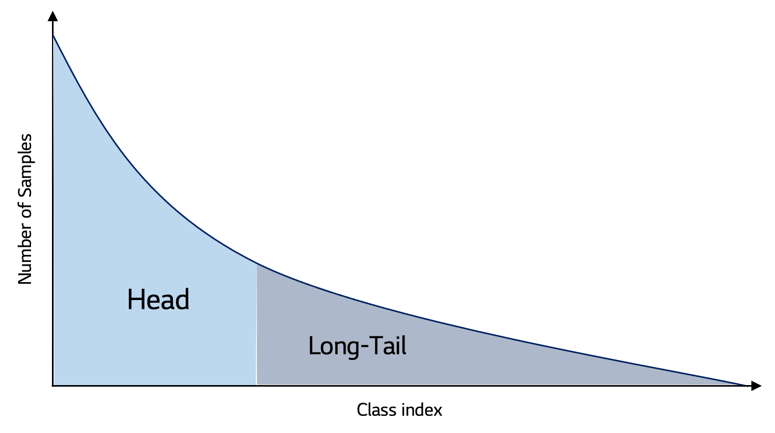
\includegraphics[width=0.8\textwidth]{Images/long_tail_distribution.png} 
    \caption{Illustration of a long-tailed distribution \cite{lgresearch257}. }
    \label{fig:lt_distribution} 
\end{figure}

\noindent A balanced dataset is one where all classes are evenly represented, whereas imbalanced datasets feature varying sample sizes across classes. Long-tailed datasets are characterized by a significant class imbalance, where a few dominant classes account for most samples (head classes), while the majority of classes are underrepresented (tail classes) as depicted in Figure \ref{fig:lt_distribution}. Mathematically, a long-tailed training set is denoted as $X=\{x_i, y_i\}_{i=1}^n$, where each sample $x_i$ has a corresponding class label $y_i$ \cite{zhang2023deep}. The total number of training samples over $K$ classes is $n = \sum_{k=1}^K n_k$, where $n_k$ represents the number of samples in class $k$. Let $\pi$ denote the vector of label frequencies, where $\pi_k = \frac{n_k}{n}$ indicates the label frequency of class $k$. It can be assumed that the classes are sorted by cardinality in decreasing order. This class distribution is common for real-world datasets \cite{Newman_2005, liu2019largescalelongtailedrecognitionopen}, for example, the iNaturalist, a popular benchmark for image classification, exhibits a long-tailed distribution of species \cite{vanhorn2018inaturalistspeciesclassificationdetection}. Other benchmarks are constructed by sampling from datasets such as ImageNet \cite{ImageNet2009} by using a Pareto distribution, which simulates long-tailed class distributions with a power-law decay \cite{zhang2023deep, dealvis2024surveydeeplongtailclassification,cao2019learningimbalanceddatasetslabeldistributionaware}.

CIFAR-100-LT \cite{cao2019learningimbalanceddatasetslabeldistributionaware}, derived from the CIFAR-100 dataset \cite{krizhevsky2009learning}, serves as the primary dataset for the experiments conducted in this thesis. CIFAR-100 is a widely used benchmark in classification research due to its diverse class representation and manageable size. It consists of 60,000 $32 \times 32$ color images divided into 100 classes, each with 600 samples. These are further split into 500 training images and 100 testing images per class. CIFAR-100-LT is created by reducing the number of samples in certain classes of CIFAR-100 following an exponential decay en sample sizes, given by:

\begin{equation}
    \label{eq:exp}
    n_i = n_{max}\cdot \text{IR}^{\frac{i-1}{K-1}}
\end{equation}

Where $n_i$ is the number of samples in class $i$, $n_{max}$ is the number of samples in the most frequent class, IR is the imbalance ratio, and $K$ is the total number of classes \cite{cao2019learningimbalanceddatasetslabeldistributionaware}.

Other long-tailed datasets follow a Pareto distribution with number of samplers per class as followed \cite{liu2019largescalelongtailedrecognitionopen}:

\begin{equation}
    \label{eq:pareto}
    f(K) = \frac{\alpha K_{\text{m}}^\alpha}{K^{\alpha + 1}}, \quad K \geq K_{\text{m}}, \quad \alpha > 0
\end{equation}

\noindent Here, $\alpha$ is the shape parameter, $K_{\text{m}}$ is the scale parameter representing the minimum possible class index, and $K$ is the class index. A larger $\alpha$ results in a more severe imbalance.



Class imbalance has a profound impact on model performance compared to evenly distributed datasets \cite{vanhorn2017deviltailsfinegrainedclassification, cui2019classbalancedlossbasedeffective}. Deep networks trained on long-tailed datasets often exhibit biased performance, favoring head classes while performing poorly on tail classes \cite{zhang2023deep}. Zhang et al. \cite{zhang2023deep} provide a comprehensive survey of methods addressing this challenge, categorizing current approaches into three main groups: class re-balancing, information augmentation, and module improvement. This thesis focus on class re-balancing methods which will be further explored in section \ref{sec:lt_methods}. 




% ===============================================================================
% Model architechtures

\section{Model Architectures}
\label{sec:model_arch}
Deep learning has revolutionized image classification by introducing models capable of learning complex patterns and representations from data. Among these, CNNs and ViTs are chosen as the primary architectures used in this thesis due to their performance on image classification tasks. This section provides a theoretical foundation for these models, focusing on the specific architectures utilized: MobileNetV2 \cite{sandler2018mobilenetv2}, ResNet-50 \cite{he2015deepresiduallearningimage}, and ConvNeXt-Base \cite{todi2023convnext} as the CNN architectures, and ViT-B/16 \cite{dosovitskiy2021imageworth16x16words} as the ViT architecture.
These models were chosen to represent a spectrum of design paradigms; from lightweight CNNs to transformers. By evaluating models of varying complexity, this study aims to identify architectures best suited for long-tailed learning under different resource constraints and data distributions.

% ===============================================================================
% DNNs

\subsection{Introduction to Deep Neural Networks}
\label{sec:intro_DNN}
Before the introduction of CNNs and, more recently, ViTs, the standard approach for image classification involved flattening a two-dimensional image matrix into a one-dimensional array and passing it through a Multilayer Perceptron (MLP), also known as a feed-forward neural network. MLPs are fully connected neural networks composed of an input layer, output layer, and one or more hidden layers, as illustrated in Figure \ref{fig:dnn_layers}. Being fully connected means that each neuron in a given layer is connected to all neurons in the next layer, forming a dense network. These connections are associated with weights and biases, which the network learns during training. Input features are fed into the input layer, propagated through hidden layers that add complexity to model nonlinear relationships, and yield predictions in the output layer. Known as universal approximators, MLPs can approximate any continuous function given sufficient neurons in the hidden layers \cite{zhang2023dive,HORNIK1989359}.

\begin{figure}[ht]
    \centering
    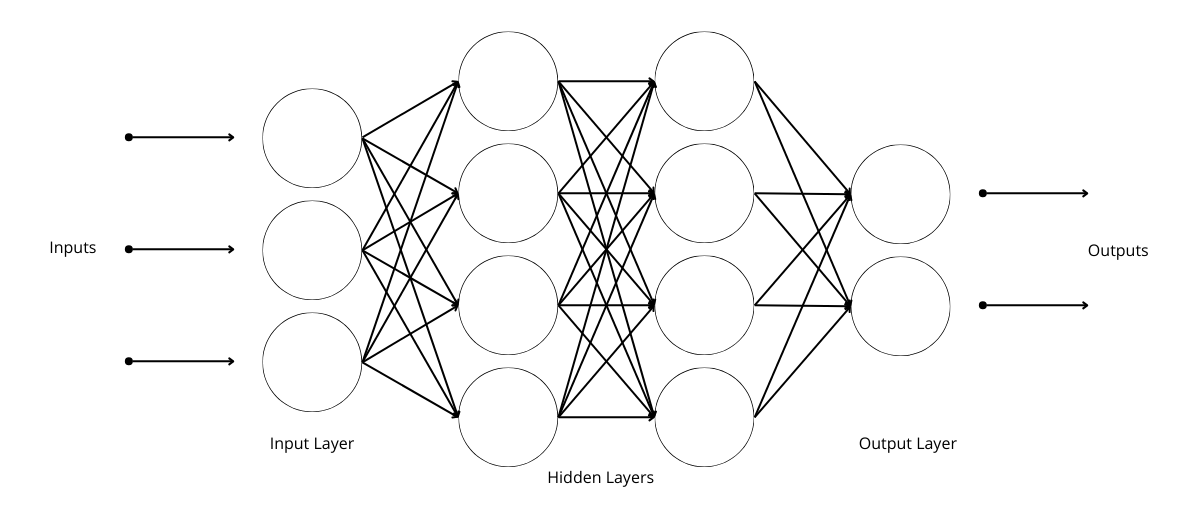
\includegraphics[width=0.8\textwidth]{Images/cnn_layers.png} 
    \caption{Layers of a neural network. This neural network consists of three input neurons, two hidden layers with four neurons each, and two output neurons. The layers are fully connected.}
    \label{fig:dnn_layers}
\end{figure}

\noindent Figure \ref{fig:dnn_layers} shows an example of a feed-forward neural network with three input neurons, two hidden layers, each with four neurons, and two output neurons. This architecture could be used, for instance, to classify images of cats and dogs based on three input features, such as height, width, and weight of the animals. The input propagates through the network, with each neuron computing a weighted sum of its inputs followed by an optional nonlinearity. The final output is a prediction, where the class corresponding to the neuron with the highest value is chosen.


However, this simple neural network becomes insufficient for more complex problems, such as image classification, as it requires an increasing number of parameters. For instance, a $224\times 224$ RGB image flattened is very large, making MLPs parameter-heavy and inefficient. The limitations of MLPs were addressed by CNNs, which introduced convolutional and pooling layers to effectively preserve and utilize the spatial information of pixels in two-dimensional images \cite{zhang2023dive}.


% ===============================================================================
% CNNs

\subsection{Convolutional Neural Networks}
\label{sec:CNNs}
CNNs \cite{lecun1995} were introduced to address the limitations of MLPs for image-related tasks. Unlike MLPs, which treat input features as independent, CNNs are designed to recognize patterns in images by applying local filters through convolutional layers, and thereby preserving the two dimensional input of an image \cite{lecun1998,NIPS2012_c399862d,zhang2023dive}. 

\begin{figure}[ht]
    \centering
    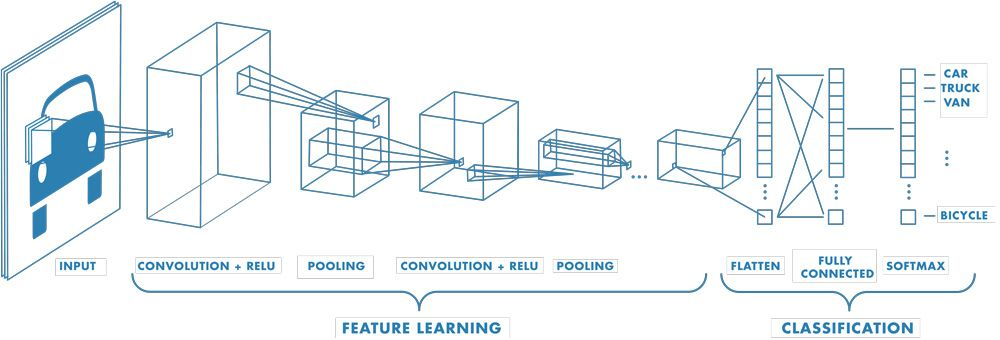
\includegraphics[width=0.8\textwidth]{Images/CNN_illustration.jpg} 
    \caption{Illustration of a convolutional neural network \cite{mathworks_cnn}.}
    \label{fig:cnn_illustration}
\end{figure}

\noindent CNNs consist of several core components, as illustrated in Figure~\ref{fig:cnn_illustration}, and have three main types of layers: convolutional layers, pooling layers, and a Fully Connected (FC) layer \cite{cs231n}. The convolutional layer is the first layer, and serves to extract local features by applying filters to small regions of an image. Pooling layers reduce the spatial dimensions of feature maps, providing invariance to small translations. CNNs are typically made of multiple convolution and pooling layers, but the final layer is the FC layer. Activation functions, such as ReLu \cite{relu},  introduce nonlinearity, allowing the network to capture complex patterns. At the final stage, FC layers aggregate the extracted features into predictions, enabling tasks such as classification or segmentation. CNNs use three-dimensional data for image classification: \emph{width}, \emph{height}, \emph{depth}. As an example, an image from the CIFAR-100 dataset has dimensions $32\times 32\times 3$, corresponding to width, height, and 3 color channels (RGB). The following provides an overview of function of the layers.

\paragraph{Convolutional Layer}
The convolutional layer is the foundation of CNNs. It applies a set of filters (called kernels) to the input image, performing convolutions to produce feature maps \cite{cs231n}. Each filter is designed to detect specific features, such as edges or textures. The filter, which has smaller dimensions than the input, is applied to an area of the image, computing dot products between the weights of the filter and the input pixels, as illustrated in figure \ref{fig:convolution}. Afterwards, the filter shifts by a stride, repeating the process until the kernel has computed the dot products for entire image. This process enables the network to learn spatial hierarchies of features, with the early layers capturing patterns like edges, and later layers capturing detailed structures \cite{yosinski2014transferablefeaturesdeepneural}. After each convolution, the ReLu transformation is applied to introduce non-linearity \cite{cs231n}.

\begin{figure}[ht]
    \centering
    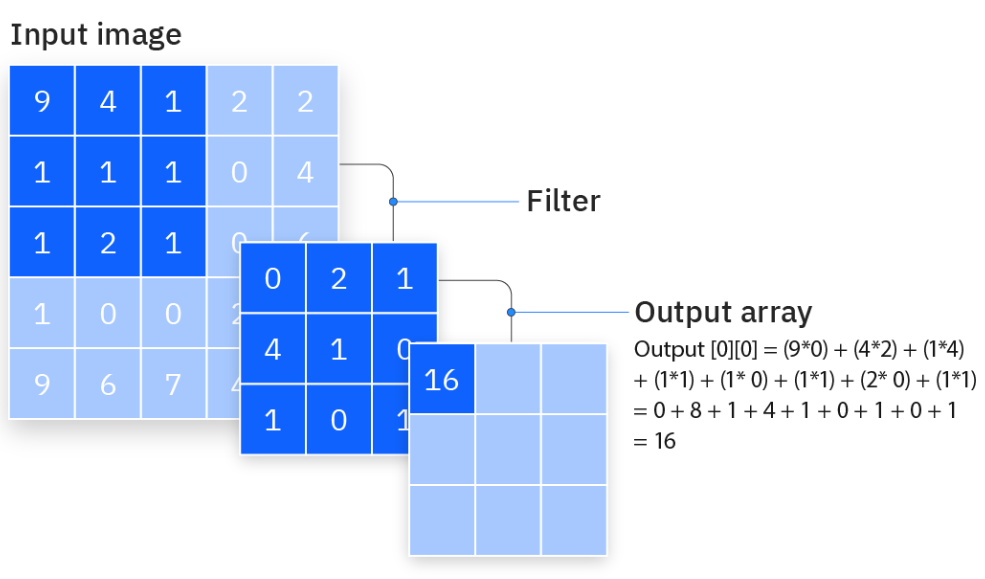
\includegraphics[width=0.6\textwidth]{Images/convolution.png} 
    \caption{Illustration of a convolution with a $3\times 3$ kernel \cite{ibm_cnn}.}
    \label{fig:convolution}
\end{figure}

\paragraph{Pooling Layer}
The function of the pooling layer (also known as downsampling) is to reduce the spatial dimensions of the feature maps, decreasing the number of parameters and computational load of the netwrok \cite{cs231n}. Moreover, this contributes to making the detection of features invariant to scale and orientation.  

\paragraph{Fully Connected Layer}
The FC layer, as the name implies, connects every neuron in one layer to every neuron in the next. Positioned at the end of the network, this performs the task of classification based on the features extracted from the previous layers \cite{cs231n}. The raw output of the FC layer are called logits \cite{arora2024logits}, and refers to the $K$-dimensional output vector for $K$ classes. These have raw outputs can range from $[-R,R]$, where $R$ are real numbers. However, an activation function must be applied to the logits to get the final probabilities of the model prediction. For multi-class classification, this activation function is the Softmax function introduced later in section \ref{sec:intro_losses}.
\vspace{1em}

\noindent These layers, combined with the architectural design of CNNs, introduce inductive biases that make them particularly well-suited for image-related tasks \cite{kim2020inductivebias}. 
% For instance, the use of convolutional filters enforces local connectivity, enabling the network to focus on localized patterns such as edges and textures. Additionally, the weight-sharing mechanism in convolutional layers provides translation invariance, allowing features to be recognized regardless of their position within the image.

% Pooling layers contribute to a spatial hierarchy, making the network robust to small positional changes and reducing computational complexity. Moreover, the multi-layered structure of CNNs facilitates hierarchical feature learning, where early layers capture simple features, and deeper layers learn increasingly complex representations. These inductive biases are fundamental to the effectiveness of CNNs in tasks like image classification and segmentation, as they align closely with the structure and characteristics of image data.


CNNs gained popularity after the introduction of LeNet-5 by LeCun et al. in 1998 \cite{lecun1998}, which showcased their capability to recognize handwritten digits. The field advanced significantly in 2012 when AlexNet \cite{NIPS2012_c399862d} won the ImageNet Challenge \cite{ILSVRC15}, demonstrating the effectiveness of deeper architectures and multi-GPU training for large-scale image recognition tasks. Subsequent developments led to influential architectures such as VGGNet \cite{simonyan2015deepconvolutionalnetworkslargescale}, GoogLeNet \cite{szegedy2014goingdeeperconvolutions}, and the state-of-the-art ResNet \cite{he2015deepresiduallearningimage}. The CNN architectures explored in this thesis are detailed in later in this section.

% ===============================================================================
% Vision Transformers

\subsection{Vision Transformers}
\label{sec:ViTs}
ViTs, introduced by Dosovitskiy et al. in 2021 \cite{dosovitskiy2021imageworth16x16words}, presented an alternative way of handling image classification by leveragering the transformer architecture. Transformers, introduced by Vaswani et al. in 2017 \cite{vaswani2023attentionneed}, was designed for Natural Language Processing (NLP), and revolutionized the deep learning field, surpassing Recurrent Neural Networks (RNNs) in NLP tasks \cite{v7labs-vit,vaswani2023attentionneed}. The transformer architecture is based on self-attention mechanism, allowing the model to selectively weigh the significance of each part of the input. As their design lack recurrence or convolutions, transformers use positional embeddings to represent the order of tokens in a sequence. 

Likewise, in ViTs, images are represented as sequences including the class label as a learnable token for classification. To start, the input image is divided into a sequence of patches, which are then flattened and linearly embedded into a vector. The spacial information is preserved by adding positional encodings to the embeddings. Next, the sequence is fed into a transformer encoder identical to that introduced by Vaswani et al., consisting of alternating layers of Multi-head self-attention (MSP) and Multi-Layer Perceptron (MLP) blocks with Layer Norm (LN) applied before every block and residual connection after every block. The final MLP layer acts as the classification head. The illustration in figure \ref{fig:vit_arch} shows the architecture of Vision Transformers.

\begin{figure}[h!]
    \centering
    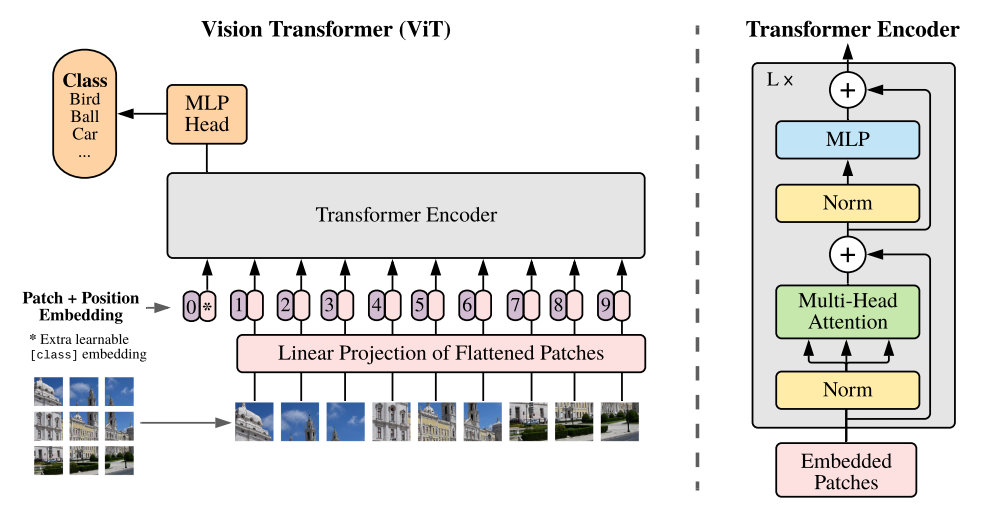
\includegraphics[width=0.8\textwidth]{Images/vision_transformer.png} 
    \caption{Vision Transformer architecture \cite{dosovitskiy2021imageworth16x16words}. The input image is split into fixed-sized patches, each liniearly embedded with added postion embedding. These are then fed to a transformer encoder.}
    \label{fig:vit_arch}
\end{figure}

\noindent Unlike CNNs, ViTs have much less image-specific inductive bias \cite{dosovitskiy2021imageworth16x16words}. While the inductive bias in CNNs help the model generalize to unseen data \cite{kim2020inductivebias}, the ViT architecture does not include built-in assumptions about the structure of the data, and only the MLP layers are local an translationally equivalent \cite{dosovitskiy2021imageworth16x16words}. As a result, ViTs require more training data to learn spacial relations compared with CNNs. However, ViTs differ from CNNs by applying self-attention mechanism across the entire image, enabling the model to capture global dependecies by attending to any patch of the image at any layer, whereas CNNs applies convolution operations over receptive fields, evolving through stacking layers \cite{cs231n}.

% \todo{What made the ViT get SOTA? Why were they better than CNNs? Scalability. \url{https://www.youtube.com/watch?v=QqejV0LNDHA}.}


% ===============================================================================
% ResNet50

\subsection{ResNet-50 Architecture}
\label{sec:resnet}
ResNet-50 is a variant of the Residual Network (ResNet) architecture, developed by Microsoft Research (He et al.) in 2015 \cite{he2015deepresiduallearningimage}. The ResNet architecture was designed to address the vanishing and exploding gradient problem in deep networks. When training a deep neural network, as the number of layers increases, the gradients of the loss function with respect to the weight can potentially vanish or explode during backpropagation \cite{he2015deepresiduallearningimage}. This can lead to slow convergence or unstable updates.

In traditional CNNs, stacked layers learn a direct mapping $\mathcal{H}(x)$ of the input $x$ to the output. The introduction of residual layers, however, allows for the layer to fit a residual mapping, as illustrated in figure \ref{fig:res_learning}, where the network learns the residual function $\mathcal{F}(x) = \mathcal{H}(x) - X$. Isolating $\mathcal{H}(x)$ yields $\mathcal{H}(x) = \mathcal{F}(x) + x$, meaning that the input $x$ is passed through a skip connection. This architecture reduces the complexity of the optimization process, as the network only has to model the residual component $\mathcal{F}(x)$ rather than the full mapping $\mathcal{H}(x)$ \cite{he2015deepresiduallearningimage}.

\begin{figure}[ht]
    \centering
    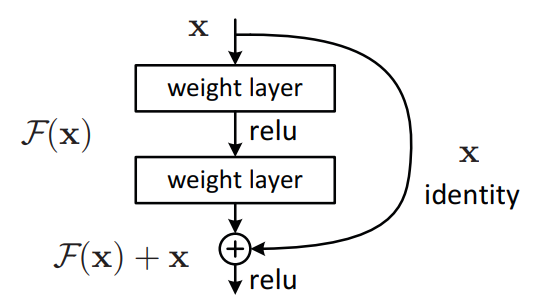
\includegraphics[width=0.5\textwidth]{Images/res_learn.png} 
    \caption{Residual learning block \cite{he2015deepresiduallearningimage}.}
    \label{fig:res_learning}
\end{figure}

\noindent The residual network is formed by stacking multiple layers of residual blocks, as the one depicted in figure \ref{fig:res_learning}. The ResNet architecture can have a varying number of layers, and, as the name implies, the ResNet-50 variant has 50 layers. Other architectures include ResNet-34, ResNet-101, and ResNet-152 \cite{he2016identitymappingsdeepresidual}. 

The ResNet-50 implementation consist of 1 convolutional layer, 4 stages of bottleneck residual blocks with layers [3, 4, 6, 3], global average pooling, and finally a fully connected layer for classification \cite{torchvision-resnet}, as seen in figure \ref{fig:resnet50}. 

\begin{figure}[ht]
    \centering
    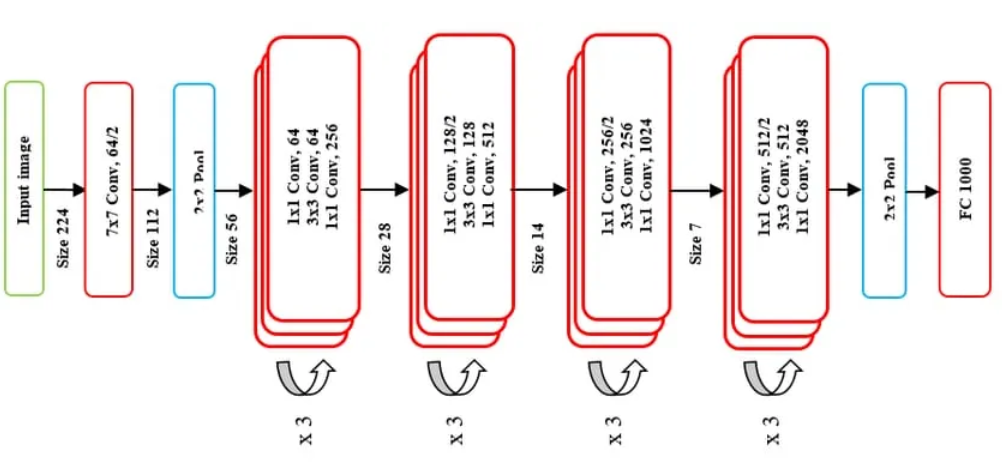
\includegraphics[width=0.7\textwidth]{Images/resnet50_blocks.png} 
    \caption{ResNet-50 architecture \cite{medium_resnet}, consisting of 6 stages: input preprocessing, 4 blocks with residual connections, and a FC layer.}
    \label{fig:resnet50}
\end{figure}

% ===============================================================================
% MobileNetV2

\subsection{MobileNetV2 Architecture}
\label{sec:mobilenet}
MobileNetV2, introduced by Sandler et al. \cite{sandler2018mobilenetv2}, is a lightweight CNN model designed primarily to balance model accuracy and computational efficiency, making it suitable for mobile or embedded devices. Building upon the original concepts of MobileNetV1 \cite{howard2017mobilenetsefficientconvolutionalneural}, MobileNetV2 preserves the use of depthwise separable convolutions, a method for reducing the parameters and floating-point operations, while introducing a novel element known as the inverted residual structure. 

% \begin{figure}[ht]
%     \centering
%     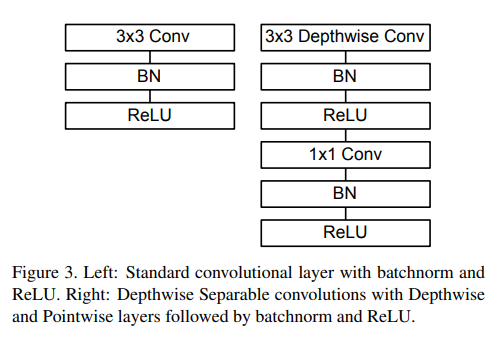
\includegraphics[width=0.8\textwidth]{Images/mobilenet_structure.png} 
%     \caption{Illustration of the MobileNetV1 structure. Figure from \cite{howard2017mobilenetsefficientconvolutionalneural}. \todo{Make this figure.}}
%     \label{fig:MobileNetV1_structure}
% \end{figure}

\paragraph{Inverted Residual Blocks}
While traditional residual connections, as described above, allow for identity mapping and improved gradient flow, MobileNetV2 employs an inverted residual structure \cite{sandler2018mobilenetv2}. Instead of mapping from a high-dimensional representation down to a lower-dimensional bottleneck, then reconstructing features at the output, inverted residual blocks begin with a low-dimensional input and expand it to a higher-dimensional space before applying a depthwise convolution. After spatial filtering, the representation is projected back down to a low-dimensional space. This approach, illustrated in Figure \ref{fig:residual}, helps preserve crucial information and maintain a rich feature space without substantially increasing computational cost. The use of a linear bottleneck (i.e., no nonlinear activation in the low-dimensional projection) also helps prevent the destruction of useful information, further improving efficiency and accuracy.  

\begin{figure}[ht]
    \centering
    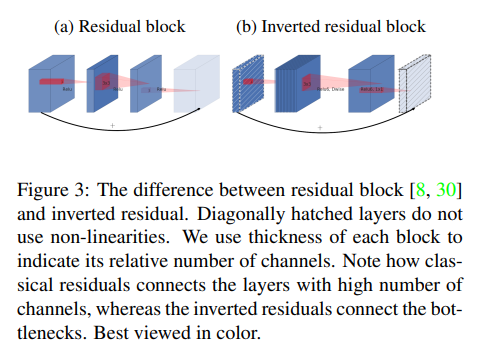
\includegraphics[width=0.8\textwidth]{Images/inverted_residual.png} 
    \caption{Residual (left) and inverted residual rlocks (right) \cite{sandler2018mobilenetv2}. The thickness of the blocks indicate their relative number of channels.}
    \label{fig:residual}
\end{figure}

\paragraph{Depthwise Separable Convolution}
Following MobileNetV1, MobileNetV2 relies on depthwise separable convolutions, depicted in Figure \ref{fig:depthwise_sep_conv}, to factorize the convolution operation into two simpler operations \cite{howard2017mobilenetsefficientconvolutionalneural}: depthwise convolution and pointwise convolution. The depthwise convolution applies a single filter to each input channel, and the pointwise convolution (a $1\times 1$ convolution) then recombines the channels to produce the desired output. In comparison, a standard convolution both filters and combines inputs into a new set of outputs. This approach reduces the parameter count and computational load, making the model suitable for devices with limited resources \cite{howard2017mobilenetsefficientconvolutionalneural,sandler2018mobilenetv2}.

\begin{figure}[ht]
    \centering
    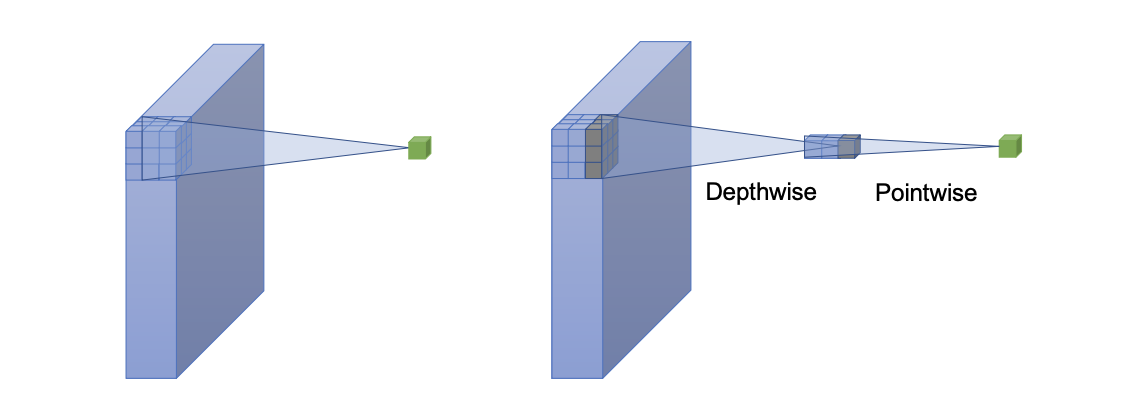
\includegraphics[width=0.8\textwidth]{Images/depthwise_separable_conv.png} 
    \caption{Standard convolution (right) and depthwise separable convolution (left) \cite{guo2019depthwiseconvolutionneedlearning}.}
    \label{fig:depthwise_sep_conv}
\end{figure}




% ===============================================================================
% ConvNeXt Base

\subsection{ConvNeXt Base Architecture}
\label{sec:convnext}
ConvNext, introduced by Liu et al. in 2022 \cite{liu2022convnet2020s}, evolutionized the traditional CNN architecture by incorporating elements from ViTs. Starting with the stem cell, the ConvNeXts employ a patchify stem, as seen in figure \ref{fig:stem}. By setting the kernel to $4 \times 4$ and the stride to 4, the result is a non-overlapping convolution where no information is shared between them, yet these are later combined in the final layers of the network.  

\begin{figure}[h!]
    \centering
    % First subfigure
    \begin{subfigure}[b]{0.45\textwidth}
        \centering
        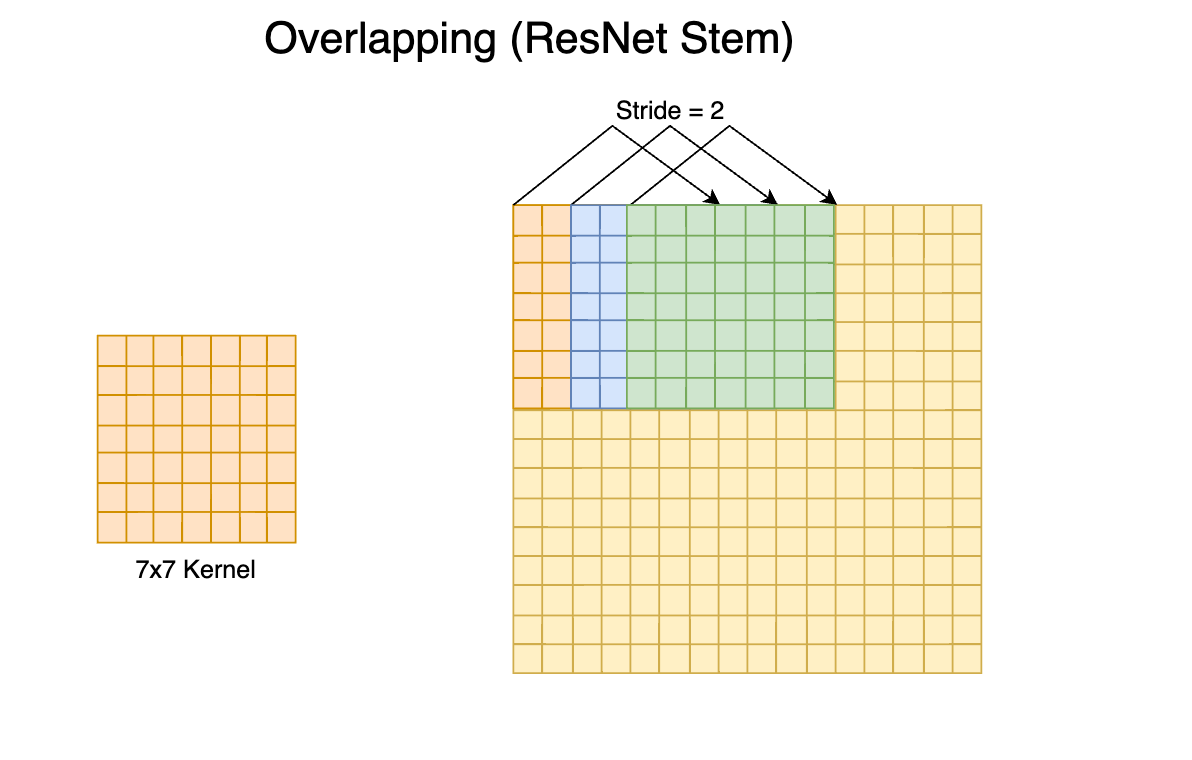
\includegraphics[width=\textwidth]{Images/cnnstem.png}
        \caption{}
        \label{fig:sub1}
    \end{subfigure}
    \hspace*{0.0\textwidth}    % Second subfigure
    \begin{subfigure}[b]{0.45\textwidth}
        \centering
        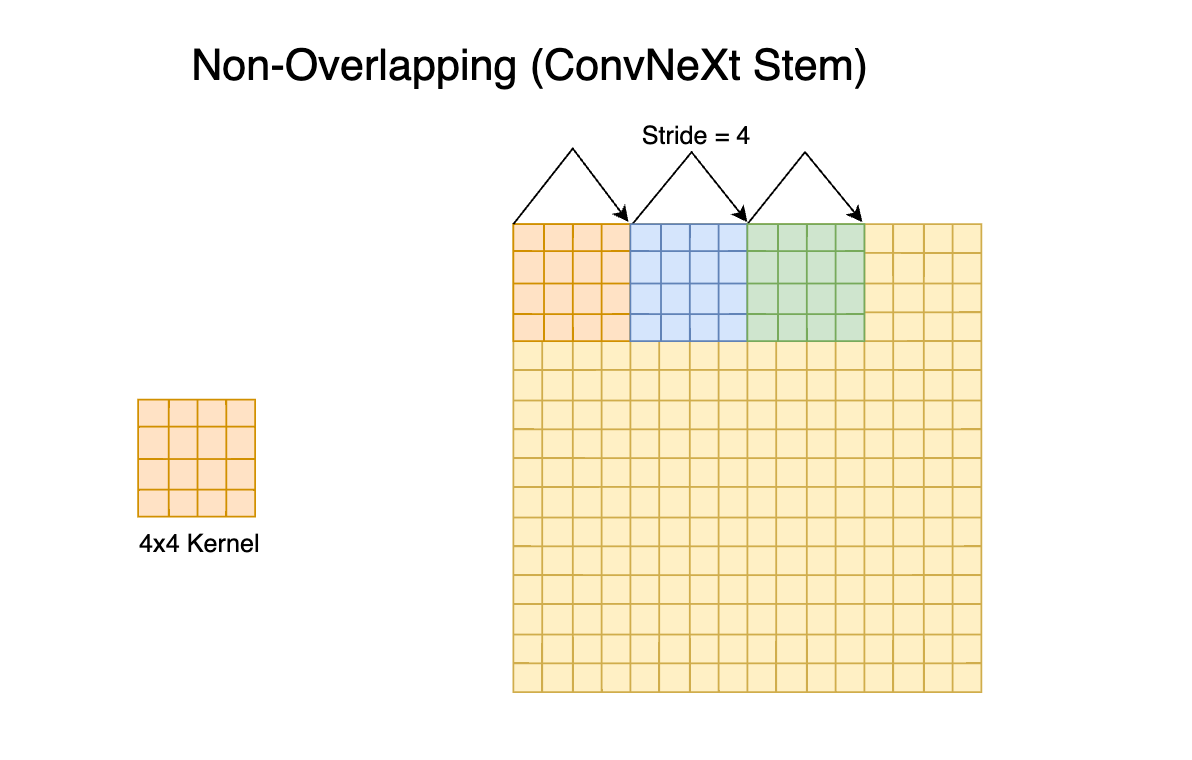
\includegraphics[width=\textwidth]{Images/convnextstem.png}
        \caption{}
        \label{fig:sub2}
    \end{subfigure}
    \caption{ResNet stem (a) vs ConvNeXt stem (b). Figure modified from \cite{convnext_guide}.}
    \label{fig:stem}
\end{figure}

\noindent Next, inspired by ResNeXt \cite{xie2017aggregatedresidualtransformationsdeep}, the ConvNeXt use depthwise convolution, already described in Section \ref{sec:mobilenet}, to increase the computation vs. accuracy trade-off. Likewise, the ConvNext incorporates inverted bottleneck blocks, which are an important design in transformers as well as MobileNetV2 \cite{liu2022convnet2020s}. Additionally, the ConvNext architecture uses a $7 \times 7$ depthwise convultion in each block on the condition of moving the depthwise convolution layer up. See figure \ref{fig:conv_block}.

\begin{figure}[h!]
    \centering
    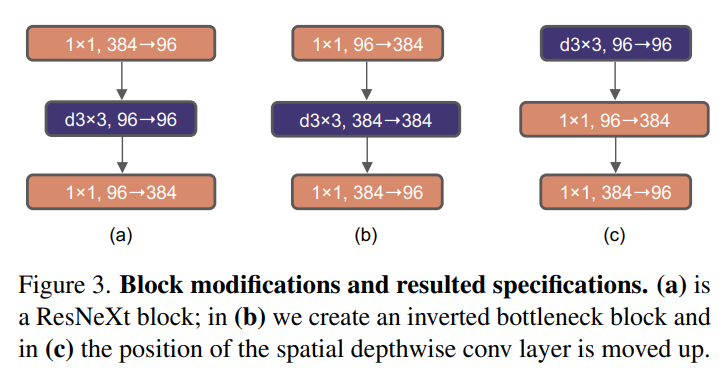
\includegraphics[width=0.6\textwidth]{Images/convnext_block_mod.png} 
    \caption{Block modifications \cite{liu2022convnet2020s}. Here, (a) is a ResNeXt block, (b) is an inverted bottleneck block, and (c) shows the position of the spatial depthwise convolutional layer moved up.}
    \label{fig:conv_block}
\end{figure}

\noindent Instead of using the ReLu activation function, commonly used in ResNets, the ConvNeXt use Gaussian Error Linear Unit (GeLU) \cite{hendrycks2023gaussianerrorlinearunits}. This activation function has shown to perform better than ReLU for transformers \cite{liu2022convnet2020s}. Additionally, ConvNext draws inspiration from transformers by removing most instances of normalization layers, only leaving them after depthwise convolutions and furhter replacing the Batch Normalization (BN) with LN. Finally, ConvNeXt introduces separate downsampling layers between blocks rather than implementing downsampling within the blocks themselves. 

These implementations has shown to improve performance, competing with ViTs \cite{liu2022convnet2020s}.

% ===============================================================================
% ViT-B/16

\subsection{ViT-B/16 Architecture}
\label{sec:vitb16}
The ViT-B/16 \cite{dosovitskiy2021imageworth16x16words} is a ViT that leverages the transformer architecture for image classification, as described in Section \ref{sec:ViTs}. One of the main characteristics of the ViT-B/16 is that the input image consist of a fixed $16 \times 16$ patch size. It has 12 stacked encoder layers, each computing self-attention with 12 heads. Additionally, each layer includes an MLP. Skip-connections are applied around self-attention and MLP blocks for better gradient flow. LN is applied before the attention and MLP blocks. Afterwards, the appended class token is extracted, and a fully connected layer maps the token to the class prediction \cite{torchvision2024vitb16}. 


%====================================================================================
% Long-Tailed Methods

\section{Class Re-balancing Methods for Long-Tailed Learning}
\label{sec:lt_methods}

Class re-balancing methods in deep learning seeks to mitigate the effects of imbalanced class distributions in training data. According to Zhang et al. \cite{zhang2023deep} class re-balancing can be divided into three sub-categories: re-sampling, class-sensitive learning, and logit adjustment. In this thesis, the primary focus is on class-sensitive learning, exploring re-weighting, re-margining, and logit adjustment strategies. For completeness, re-sampling is briefly introduced as well.


\subsection{Re-Sampling}
\label{sec:re-sampling}
Deep networks are commonly trained with mini-batch gradient descent using random sampling, i.e. each sample has an equal probability of being selected \cite{zhang2023deep}. When classes are imblanced, samples from head classes naturally occur more often, thus having higher chances of being selected than samples from tail classes, resulting in a bias towards head classes. Re-sampling addresses this problem by adjusting the sample probabilites or the sample counts per class (e.g. oversampling minority classes or undersampling majority classes). While this approach seems simple and intuitive, re-sampling can lead to overfitting of tail classes or underperformance on head classes, hence the need for more sophistacated approaches \cite{zhang2023deep}.

\subsection{Class-Sensitive Learning}
\label{sec:class-sensitive-learning}

Traditional training methods using the standard loss function, cross-entropy loss, can lead the model to be biased towards head classes, as the loss ignores class imbalance and thus generate an uneven amount of gradients for different classes \cite{zhang2023deep}, as described later in this section. Consequently, tail classes are often misclassified. To address this imbalance, class-sensitive learning methods modify the loss function to pay more attention to minority classes, thus improving performance on tail classes.

The three sub-categories of class-sensitive learning explored in this thesis are described in the following.

\subsubsection{Re-Weighting}
\label{sec:re-weighting}
Modifies the loss function, commonly the cross-entropy loss, by assigning different weights to each class \cite{zhang2023deep}. Classes with fewer samples are assigned greater weights, thus re-balancing the training process.

\subsubsection{Re-Margining}
\label{sec:re-margining}
Re-margining aims to solve class imbalance by introducing margin between classes, encouraging higher margins between rare classes. 

Figure \ref{fig:decision_boundaries} illustrates how the margin affects the decision boundary for binary classification. Here, the margin $\gamma_i$ of the $i$-th class is the minimum distance of the data in the $i$-th class to the decision boundary.  By increasing the margin, the decision boundary separates the regions of input space corresponding to different class predictions, thus the model becomes more confident in classification \cite{cao2019learningimbalanceddatasetslabeldistributionaware}.


\begin{figure}[ht]
    \centering
    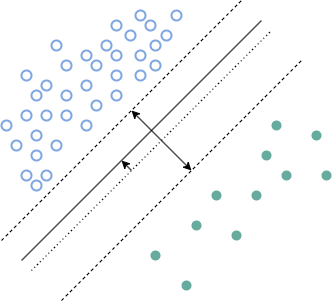
\includegraphics[width=0.3\textwidth]{Images/margin.drawio.png} 
    \caption{The margins and decision boundary of binary classification. The distance between the classes is fixed, but shifting the decision boundary can optimize the trade-off between them. \cite{cao2019learningimbalanceddatasetslabeldistributionaware}.}
    \label{fig:decision_boundaries} 
\end{figure}

% \noindent The margin is defined as:

% \begin{equation}
%     \label{eq:margin_def}
%     \gamma(x,y) = f(x)_y - \max_{j \neq y}f(x)_j
% \end{equation}

% \noindent which is the distance between the prediction of the sample $(x,y)$ and the decision boundary. The training margin for class $j$ is defined as:

% \begin{equation}
%     \label{eq:margin_class_def}
%     \gamma_j = f(x)_y - \max_{i \in S_j}\gamma(x_i,y_i)
% \end{equation}

% \noindent The classical generalization bound is defined as:

% \begin{equation}
%     \label{eq:gen_bound}
%     \text{imbalanced test error}\lesssim \frac{1}{\gamma_{min}}\sqrt{\frac{C(\mathcal{F})}{n}}
% \end{equation}

% \noindent In a balanced setting:

% \begin{equation}
%     \frac{1}{2}\text{err}[\text{class1}]+\frac{1}{2}\text{err}[\text{class2}] \lesssim \left(\frac{1}{\gamma_1\sqrt{n_1}}+\frac{1}{\gamma_2\sqrt{n_2}}\right)\sqrt{C(\mathcal{F})}
% \end{equation}

Cao et al. \cite{cao2019learningimbalanceddatasetslabeldistributionaware} has shown that the optimal margin for a class is inversely proportional to the fourth root of its frequency $n_i$, allowing the model to generalize better in imbalance settings:

\begin{equation}
    \label{eq:opt_margin}
    \gamma_i\varpropto n^{-1/4}_i 
\end{equation}

\noindent with the standard solution being $\gamma_1=\gamma_2$. 

\subsubsection{Logit Adjustment}
\label{sec:logit_adjustment}
Logit adjustment is a class re-balancing technique that aims to optimize the class imbalance by adjusting the model outputs, i.e. logits, based on prior class probabilities \cite{menon2021longtaillearninglogitadjustment,ren2020balancedmetasoftmaxlongtailedvisual}.

In classification tasks, model outputs $\eta_j$ for class $j$ are computed by:

\begin{equation}
    \label{eq:logits}
    \eta_j = \theta^T_j f(x)
\end{equation}

\noindent where $\theta_j$ are the weights for the final layer for class $j$, and $f(x)$ is the feature extractor function \cite{ren2020balancedmetasoftmaxlongtailedvisual}. Logit adjustment modifies these logits accounting for the prior class probabilites, thus shifting the model's prediction toward a more balanced output distribution \cite{ren2020balancedmetasoftmaxlongtailedvisual}.
\vspace{1em}

\noindent In the following section, the theory behind representative loss functions commonly used in class-sensitive learning is presented, beginning with an introduction to loss functions followed by the baseline CE loss. 
% Subsequently, the theory behind multiple re-weighting schemes including Weighted Softmax Cross-Entropy, Focal Loss, Class-Balanced Loss, Balanced Softmax Loss, and Equalization Loss, as well as the re-margining method LDAM Loss. Each of these methods seeks to improve the imbalance in training through modifications that ultimately improve the classification performance on tail classes.

\section{Loss Functions}
\label{sec:intro_losses}
Loss functions are a fundamental component in deep learning, as they serve as a measure of how far model predictions deviate from the actual values \cite{Goodfellow-et-al-2016,zhang2023dive}.

During training, an optimization algorithm iteratively updates the model parameters (weights and biases) with the goal of minimizing the loss using the gradient of the loss function with respect to each parameter to determine how the parameter affects the loss \cite{Goodfellow-et-al-2016}. Consequently, the loss function influences the model's interpretation of prediction errors and guides parameter updates. This process continues until the model converges or meets a stopping criterion. The experiments in this thesis are conducted using the Adam optimizer introduced by Kingma et al. \cite{kingma2017adammethodstochasticoptimization}.

For image classification tasks, the standard loss function is the cross-entropy loss combined with the softmax activation function \cite{zhang2023dive} described in the following.
% Afterwards, the model update its parameter to reduce the loss, following:

% \begin{equation}
%     \label{eq:gradient_update}
%     w_{t+1} = w_t - \eta \frac{\partial L}{\partial w_t}
% \end{equation}

% Here, $w$ are the parameters, $\eta$ is the learning rate, and $L$ is the loss function. This is an iterative process, and continues until the loss reaches a minimum or the model converges.

% \todo{This is the SGD. Include the Adam Optimizer.}
% The Adam optimizer introduced by Kingma et al. \cite{kingma2017adammethodstochasticoptimization} 
% Adam is a replacement optimization algorithm for stochastic gradient descent for training deep learning models.
% Adam combines the best properties of the AdaGrad and RMSProp algorithms to provide an optimization algorithm that can handle sparse gradients on noisy problems.
% Adam is relatively easy to configure where the default configuration parameters do well on most problems.

\subsection{Softmax Activation Function}
\label{sec:softmax}
The softmax function transforms the raw output scores (logits) of the final layer of a neural network into a probability distribution over \( K \) classes. For an input \( \mathbf{z} = [z_1, z_2, \dots, z_K] \), the softmax function is defined as:

\begin{equation}
    \label{eq:softmax}
    P(y = i \mid \mathbf{z}) = \frac{\exp(z_i)}{\sum_{j=1}^{K} \exp(z_j)}
\end{equation}

\noindent These probabilities $P(y=i)$ sum to 1, and allows the network's outputs to represent the model's confidence in each class.

\subsection{Cross-Entropy Loss}
\label{sec:ce_loss}
The CE loss is a fundamental building block in training deep classifiers and is widely regarded as the baseline in classification tasks \cite{zhang2023deep, cs231n, pytorch_crossentropy}. The CE loss combines the cross-entropy loss and the softmax activation function, and thus is commonly referred to as the \emph{Softmax Loss} \cite{zhang2023dive,Goodfellow-et-al-2016,zhang2023deep}. 

The CE loss measures the difference between the predicted probability distribution $P$ and the true class label $y$. For a single sample, the loss is defined as \cite{zhang2023dive,cs231n}:

\begin{equation}
    \label{eq:ce_multi}
    \mathcal{L}_{\text{CE}} = -\sum_{i=1}^{K} y_i \log(p_i)
\end{equation}

\noindent where $y_i$ is the ground truth label, represented as a one-hot encoded vector, and $p_i$ is the predicted probability for class $i$. This simplifies for a single ground truth class $y$:

\begin{equation}
    \label{eq:ce_single}
    \mathcal{L}_{\text{CE}} = - \log(p_y)
\end{equation}

\noindent Inserting the softmax probabilites from Eq. \eqref{eq:softmax} yields:

\begin{equation}
    \label{eq:ce_loss}
    \mathcal{L}_{\text{CE}} = - \log\left(\frac{\exp(z_y)}{\sum_{j=1}^{K} \exp(z_j)}\right)
\end{equation}

\noindent where $y$ is the true class. This equation penalizes incorrect predictions by heavily weighting the log of the predicted probability for the true class. The loss is minimized when the predicted probability \( P(y = c \mid \mathbf{z}) \) approaches 1, indicating high confidence in the correct class.

The standard CE loss (eq. \eqref{eq:ce_loss}) estimates class probabilities based on the assumption that the training and validation labels follow the same distribution, $p(y=j)$, in other words how common is the label $j$ in the data \cite{ren2020balancedmetasoftmaxlongtailedvisual}. When training with an imbalanced dataset the estimated probabilities $\phi$ can become biased when applied to data with a different class distribution, e.g. a balanced test set, which can lead to errors in predictions.

% \subsubsection{Summary of Class Re-Balancing}
% Long-tailed or imbalanced datasets pose significant challenges in classification tasks, as models trained naively tend to bias toward majority classes. Class re-balancing strategies tackle this by either sampling differently (re-sampling), adjusting the loss function to emphasize minority classes (cost-sensitive re-weighting and margin-based losses), or modifying logits based on class priors (logit adjustment). These techniques all aim to improve performance on tail classes without excessively sacrificing performance on head classes. The following sections detail how each method is applied and evaluated in the context of this thesis.

\subsection{Weighted Softmax Cross-Entropy Loss}
\label{sec:wce_loss}
The WCE loss modifies the standard CE loss (Eq. \eqref{eq:ce_loss}) by introducing a weighting factor $w$. For multiclass classification, the CE loss it is multiplied by the inverse class frequencies $1/\pi_y$ \cite{zhang2023deep,lin2018focallossdenseobject}, given by:

\begin{equation}
    \label{eq:wce_loss}
    \mathcal{L}_{\text{WCE}} = -w \log(p_y) = - \frac{1}{\pi_y} \log(p_y)
\end{equation}

\noindent This WCE loss ensures that minority classes contribute more to the overall loss, addressing the imbalance during training.


\subsection{Focal Loss}
\label{sec:fl}
FL \cite{lin2018focallossdenseobject} addresses class imbalance by improving model performance on hard-to-classify examples by focusing on wrongly classified examples. The technique for this is called down-weighting, and uses the prediction probabilities to dynamically adjust the contribution of each sample to the loss. Well-classified examples with high probabilities $p_y$ are down-weighted by adding a modulating factor $(1 - p_y)^\gamma$ to the cross-entropy loss (eq. \eqref{eq:ce_loss}). Here, $\gamma \geq 0$ is a tunable focusing parameter. The FL modifies the CE loss by applying the inverse prediction probability as follows:

\begin{equation}
    \label{eq:focal_loss}
    L_{fl} = -(1 - p_y)^\gamma \log(p_y)
\end{equation}

\noindent This factor increases the weight of misclassified examples, ensuring the model prioritizes learning from challenging samples. Figure \ref{fig:focal_loss} shows how the focal loss for different values of $\gamma$. When $\gamma = 0$ the modulating factor equals 1, and the focal loss becomes the standard CE loss. The blue line in figure \ref{fig:focal_loss} represents the standard cross-entropy loss for $\gamma = 0$.

\begin{figure}[h!]
    \centering
    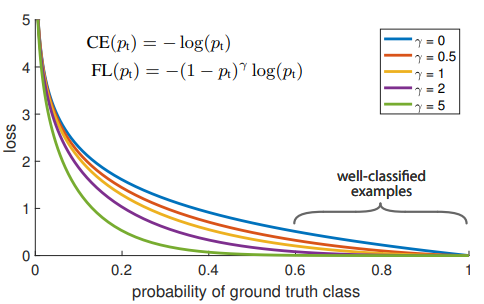
\includegraphics[width=0.6\textwidth]{Images/focal_loss.png}
    \caption{Focal loss for various values of $\gamma$. \cite{lin2018focallossdenseobject}.}
    \label{fig:focal_loss}
\end{figure}

\subsection{Class-Balanced Loss}
\label{sec:cb_loss}
CB loss \cite{cui2019classbalancedlossbasedeffective} introduces a re-weighting strategy based on the effective number of samples per class to re-balance the loss. Instead of simply using raw class frequencies, CB loss estimates how much additional information new samples provide, acknowledging an information overlap among data, and as the number of samples increases, the marginal benefit of extracted features from new data diminishes. As illustrated in figure \ref{fig:cb_featue_space}, the feature space is the map of all possible data, and each sample occupies a part of the space. Collecting more samples of a class means that there is a probability that their features overlap, meaning that additional samples diminishes new information.
In feature space, the probability of newly sampled data with volume 1 is overlapping $p$, which means that the probability of adding new information to the feature space is $(1-p)$. 


\begin{figure}[h!]
    \centering
    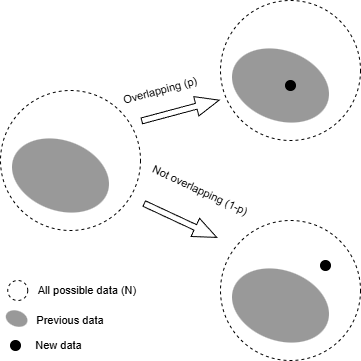
\includegraphics[width=0.5\textwidth]{Images/featurespace.drawio.png}
    \caption{The probability of newly sampled data (black dot) to overlap with previously samples data (grey area) given the set of all possible data (dashed circle). \cite{cui2019classbalancedlossbasedeffective}.}
    \label{fig:cb_featue_space}
\end{figure}

\noindent Cui et al. \cite{cui2019classbalancedlossbasedeffective} introduced the effective number of samples as the expected volume of samples, denoted $E_n$, where $n \in \mathbb{Z}_{>0}$ is the number of sampels. The effective number of samples 
is defined as:

\begin{equation}
    \label{eq:eff_num}
    E_n = \frac{1-\beta^n}{1-\beta}
\end{equation}

\noindent where $\beta = (N-1)/N$. The hyperparameter $\beta \in [0,1)$ determines how fast $E_n$ grows.

As a result, the CB loss introduces a class-balanced re-weighting term, inversely proportional to the effective number of classes. Adding the CB term to the standard softmax cross-entropy given in Eq. \eqref{eq:ce_loss} yield the following:

\begin{equation}
    \label{eq:cb_loss}
    L_{cb} = - \frac{1 - \beta}{1 - \beta^{n_y}} \log(p_y)
\end{equation}

\noindent where $n_y$ is the number of samples in the ground truth class $y$. Applying the inverse of the effective number ensures that minority classes contribute more to the total loss, as the effective number in Eq. \eqref{eq:eff_num} grows large for minority classes (small $n_y$) and small for majority classes (large $n_y$). When $\beta = 0$ the loss is equivalent to the CE loss. Contrary, when $\beta \longrightarrow 1$ the re-weighting effect grows.


\subsection{Softmax Equalization Loss}
\label{sec:seql}
Equalization Loss (EQL) \cite{tan2020equalizationlosslongtailedobject} aims to mitigate the over-suppression of tail classes, which occurs when underrepresented classes serve predominantly as negative examples for the more frequent classes. The idea is to ignore the gradients for rare classes so that they are not excessively penalized when they appear as negatives, preventing their learned representations from being overshadowed. An analysis of gradient impact on classes is seen in figure \ref{fig:eql_gradients}.

\begin{figure}[ht]
    \centering
    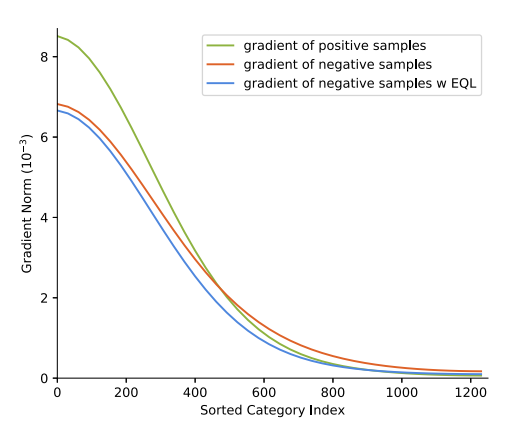
\includegraphics[width=0.6\textwidth]{Images/gradient_analysis.png} 
    \caption{Gradient analysis on positive and negative examples along with negative samples with Equalization Loss \cite{tan2020equalizationlosslongtailedobject}.}
    \label{fig:eql_gradients} 
\end{figure}

\noindent The EQL was designed for object recognition, but the authors decided to adopt the principles into image classification, officially called the \emph{Softmax Equalization (SEQ) Loss}, defined as: 

\begin{equation}
    \label{eq:EQ_loss}
    \mathcal{L}_{SEQL} = - \sum_{j=1}^{C} y_j \log(\tilde{p}_j)
\end{equation}

\noindent where

\begin{equation}
    \tilde{p}_j = \frac{e^{z_j}}{\sum_{k=1}^{C} \tilde{w}_k e^{z_k}}
\end{equation}

\noindent and the weight term is given by:

\begin{equation}
    \tilde{w}_k = (1 - \beta T_\lambda(f_k))(1 - y_k)
\end{equation}

\noindent Here, $y_j$ is the ground truth class, $z_j$ is the logit for class $j$, $f_k$ is the frequency of class $k$, \(T_\lambda(\cdot)\) is the threshold on class frequency. As there is no background category for image classification tasks, $\beta$ is introduced to randomly maintain the gradient of negative samplers. \(\beta\) is a random variable with probability \(\gamma\) of taking value 1 and probability \(1 - \gamma\) of taking value 0.


\subsection{Balanced Softmax Loss}
\label{sec:bs_loss}
The \emph{Balanced Softmax (BS)} Loss modifies the standard softmax loss (eq. \eqref{eq:ce_loss}) by directly incorporating class priors $\pi_y$ into the logits before computing probabilities \cite{ren2020balancedmetasoftmaxlongtailedvisual}. Unlike approaches that operate solely in the loss space, BS Loss integrates class frequency adjustments at the probability computation stage, effectively neutralizing the bias introduced by imbalanced class distributions. 

Ren et al. \cite{ren2020balancedmetasoftmaxlongtailedvisual} introduces Softmax regression as a multinomial distribution, $\phi$, dependent on $\eta$, defined as:

\begin{equation}
    \phi_j = \frac{e^{\eta_j}}{\sum_{i=1}^{k}e^{\eta_i}}
\end{equation}

\noindent where $k$ are the number of classes.

The Balanced Softmax uses the output logits $\eta$ (Eq. \eqref{eq:logits}) to parametize two separate probabilities: $\phi$ for testing, and $\hat{\phi}$ for training. This separation is used when training with an imbalanced dataset to eliminate the discrepancy between training and testing distributions \cite{ren2020balancedmetasoftmaxlongtailedvisual}.

Assume $\phi$ to be the desired conditional probability of the balanced dataset, with the form $\phi_j = p(y = j \mid x) = \frac{p(x \mid y=j)}{p(x)} \cdot \frac{1}{k}$, and $\hat{\phi}$ to be the desired conditional probability of the imbalanced training set, with the form $\hat{\phi}_j = \hat{p}(y = j \mid x) = \frac{p(x \mid y=j)}{\hat{p}(x)} \cdot \frac{n_j}{\sum_{i=1}^{k} n_i}$. If $\phi$ is expressed by the standard Softmax function of the model output $\eta$, then $\hat{\phi}$ can be expressed as:

\begin{equation}
    \hat{\phi}_j = \frac{n_j e^{\eta_j}}{\sum_{i=1}^{k} n_i e^{\eta_i}}.
\end{equation}

\noindent where $n_j$ is the number of samples in class $j$.

Ren et al. \cite{ren2020balancedmetasoftmaxlongtailedvisual} proved that this method can accomodate the label distribution shifts between training and test sets \cite{ren2020balancedmetasoftmaxlongtailedvisual}. Ultimately, the Balanced Softmax loss function is becomes:

\begin{equation}
    \mathcal{L}_{bs} = - \log\left( \frac{\pi_y \exp(z_y)}{\sum_j \pi_j \exp(z_j)} \right)
\end{equation}

\noindent where $z_y$ represents the logit for the true class, $\pi_y$ is the class prior (e.g. normalized frequency of samples from class $y$), and the term in the denominator normalizes the probabilities across all classes while accounting for priors.




\subsection{LDAM Loss}
\label{sec:ldam_loss}
The \emph{Label-Distribution-Aware Margin (LDAM)} Loss \cite{cao2019learningimbalanceddatasetslabeldistributionaware} represents a class-sensitive approach based on re-margining. Instead of altering the loss directly, LDAM modifies the margin applied to each class' decision boundary, ensuring that the model is more confident in classification for minority classes. The goal is to apply the optimal boundary in Eq. \eqref{eq:opt_margin} by increasing the distance between the largest and second largest logit for each class and introducing that to the cross-entropy loss (eq. \eqref{eq:ce_loss}).


The class-dependent margin for multiple classes is defined as:

\begin{equation}
    \label{eq:margin}
    \gamma_j = \frac{C}{n^{1/4}_j}
\end{equation}

\noindent where $C$ is a tunable hyper-parameter, and $n_j$ is the number of samples in class $j$. Applying the margin through the loss function, inspired by the Hinge Loss \cite{cao2019learningimbalanceddatasetslabeldistributionaware}, will encourage the model to respect the margins in Eq. \eqref{eq:margin}:

\begin{equation}
    \label{eq:ldam-hg}
    \mathcal{L}_{ldam-hg} = \max\left(\max_{j \neq y}\{z_j\} - z_y + \Delta_y, 0\right)
\end{equation}

\noindent where

\begin{equation}
    \Delta_j = \frac{C}{n_j^{1/4}} \quad \text{for } j \in \{1, \dots, k\}.
\end{equation}

\noindent and $z_y$ is the model output (logit) for the true class $y$, and $\max_{j \neq y}\{z_j\}$ is the highest score among incorrect classes. Adding the margin $\Delta_j$ ensures that the true class logit is separated from the highest incorrect score by the at least $\Delta_j$. However, since the function in Eq. \eqref{eq:ldam-hg} is non-differentiable at certain points, a modifications to the cross-entropy loss is used to address this. Here, the class-dependent margins are introduced directly into the logits as follows:

\begin{equation}
    \label{eq:ldam}
    L_{ldam} = - \log\left( \frac{\exp(z_y - \Delta_y)}{\sum_j \exp(z_j - \Delta_j)} \right)
\end{equation}